\documentclass[]{article}
\usepackage[UTF8]{ctex}
\usepackage[a4paper,left=10mm,right=10mm,bottom=10mm,top=10mm]{geometry}
\usepackage{graphicx}
\usepackage{float}
\usepackage{amsmath,amsfonts,amssymb,amsthm}
\usepackage{array,color}
%opening
\title{计算机科学中的数学基础-Exercise5}
\author{陈昱衡 521021910939}
\date{}

\begin{document}

\maketitle

\section*{Warmup7}
\begin{figure}[H]
    
\includegraphics[scale = 1]{Q1.png}
\end{figure}
分局m次上升幂的定义,将式子展开,有,
\begin{equation}
    % \bigtriangledown
    \bigtriangledown{(x^{\bar{m}})} = x^{\bar{m}} - (x-1)^{\bar{m}}
\end{equation}
展开,
\begin{align}
    =&x(x+1)(x+2)\cdots(x+m-1)-(x-1)x(x+1)\cdots(x+m-2) \\
    =&x(x+1)\cdots(x+m-2) \times (x+m-1-(x-1))\\
    =&mx(x+1)\cdots(x+m-2)\\
    =&m(x-1)^{\overline{m-1}}
\end{align}

\section*{Warmup8}
\begin{figure}[H]
    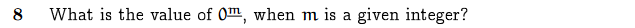
\includegraphics[scale = 1]{Q2.png}
\end{figure}
对m的取值范围分类讨论,有,\par 
若m$ \ge$ 0,
\begin{align}
    0^{\underline{m}} &= 0 \times 1 \times \cdots (m-1)\\
                        & =0
\end{align}
若 m < 0,
\begin{align}
    0^{\underline{m}} &= \frac{1}{1\times 2 \times \cdots m}\\
                        &=\frac{1}{|m|!}
\end{align}

\section*{Warmup9}
\begin{figure}[H]
    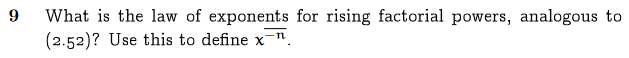
\includegraphics[scale = 1]{Q3.png}
\end{figure}
类比2.52:
\begin{equation}
    x^{\underline{m+n}} = x^{\underline{m}}(x-m)^{\underline{n}}
\end{equation}
可得:
\begin{equation}
    x^{\bar{m+n}} = x^{\bar{m}}(x+m)^{\bar{n}}
\end{equation}
对上式,令m=-n,就有:
\begin{align}
    1 &= x ^ {\overline{-n}} \times (x-n) ^ {\bar{n}}\\
    x & ^ {\overline{-n}} = \frac{1}{(x-n) ^ {\bar{n}}}  \\
    x & ^ {\overline{-n}} = \frac{1}{(x-1)^{\underline{n}}}
\end{align}

\section*{Warmup10}
\begin{figure}[H]
    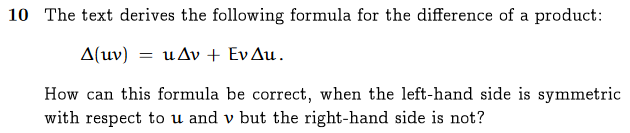
\includegraphics[scale = 1]{Q4.png}
\end{figure}
由推导:
\begin{align}
    \Delta(u(x)v(x))=&u(x+1)v(x+1)-u(x)v(x)\\
    =&u(x+1)v(x+1)-u(x)v(x+1)+u(x)v(x+1)-u(x)v(x)\\
    =&u(x)\Delta v(x)+v(x+1)\Delta u(x)
\end{align}
可知,左侧同样等于:
\begin{align}
    \Delta(u(x)v(x))=&u(x+1)v(x+1)-u(x)v(x)\\
    =&u(x+1)v(x+1)-u(x+1)v(x)+u(x+1)v(x)-u(x)v(x)\\
    =&u(x+1)\Delta v(x)+v(x)\Delta u(x)
\end{align}
即,
\begin{equation}
    \Delta (uv)=Eu\Delta v +v \Delta u
\end{equation}

\section*{Basic14}
\begin{figure}[H]
    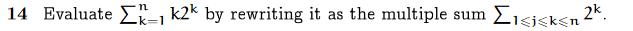
\includegraphics[scale = 1]{Q5.png}
\end{figure}
显然,
\begin{equation}
    k=\sum_{j=1}^{k}
\end{equation}
故,原式等于,
\begin{align}
    \sum_{k=1}^{n}k2^k&=\sum_{k=1}^{n}\sum_{j=1}^{k}2^k\\
                    &=\sum_{1 \le j \le n} (2^{n+1} - 2^{j})\\
                    & = n2^{n+1} - (2^{n+1} -2) \\
                    &=(n-1)2^{n+1} -2
\end{align}

\end{document}